\documentclass[slidescentered]{beamer}
\usepackage[english]{babel}
\usepackage[utf8x]{inputenc}
\usepackage[T1]{fontenc}
\usepackage{color}
\usepackage{graphicx}

\usetheme{UniboTesi}

\title{Machine Learning Project}
\subtitle{Bank Marketing Binary Classification}
\date{\today}
\department{Computer Science and Engineering}
\degree{Master Degree in Artificial Intelligence}

\begin{document}

%------------------------------------------------
\begin{frame}[noframenumbering]
\titlepage
\end{frame}

%------------------------------------------------
\begin{frame}{Project Objective}
\begin{itemize}
\item Predict whether a client subscribes to a term deposit.
\item Binary classification on a bank marketing dataset.
\item Goal: maximize ROC-AUC score on Kaggle leaderboard.
\item Dataset size: 
\begin{itemize}
\item Train: 750k rows, 18 features
\item Test: 250k rows
\end{itemize}
\end{itemize}
\end{frame}

%------------------------------------------------
\begin{frame}{Dataset Description}
Features include:
\begin{itemize}
\item Client data: age, job, marital status, education
\item Financial info: balance, housing loan, personal loan
\item Campaign info: duration, pdays, campaign, previous contacts
\end{itemize}
Target:
\begin{itemize}
\item y = subscription to term deposit
\end{itemize}
\end{frame}

\begin{frame}{Dataset Preview}{First 5 rows of the Bank Dataset}
    \begin{center}
    \tiny
    \addtolength{\tabcolsep}{-4pt} % Adjust column spacing to fit
    \begin{tabular}{|l|c|c|l|l|l|c|c|c|c|c|c|c|c|c|c|c|c|c|}
    \hline
    \textbf{} & \textbf{id} & \textbf{age} & \textbf{job} & \textbf{marital} & \textbf{educ.} & \textbf{def.} & \textbf{bal.} & \textbf{hous.} & \textbf{loan} & \textbf{cont.} & \textbf{day} & \textbf{mon.} & \textbf{dur.} & \textbf{cam.} & \textbf{pday} & \textbf{prev.} & \textbf{pout.} & \textbf{y} \\ \hline
    0 & 0 & 42 & techn. & married & sec. & no & 7 & no & no & cell. & 25 & aug & 117 & 3 & -1 & 0 & unk. & 0 \\ \hline
    1 & 1 & 38 & blue-c. & married & sec. & no & 514 & no & no & unk. & 18 & jun & 185 & 1 & -1 & 0 & unk. & 0 \\ \hline
    2 & 2 & 36 & blue-c. & married & sec. & no & 602 & yes & no & unk. & 14 & may & 111 & 2 & -1 & 0 & unk. & 0 \\ \hline
    3 & 3 & 27 & student & single & sec. & no & 34 & yes & no & unk. & 28 & may & 10 & 2 & -1 & 0 & unk. & 0 \\ \hline
    4 & 4 & 26 & techn. & married & sec. & no & 889 & yes & no & cell. & 3 & feb & 902 & 1 & -1 & 0 & unk. & 1 \\ \hline
    5 & 5 & 24 & admin. & single & sec. & no & 1882 & yes & no & cell. & 20 & apr & 1010 & 3 & -1 & 0 & unk. & 0 \\ \hline
    \end{tabular}
    \end{center}

    \vspace{0.5cm}
    \begin{itemize}
        \item \textbf{Target variable (y):} 0 = No subscription, 1 = Subscription.
        \item Large variety of categorical and numerical features.
    \end{itemize}
\end{frame}



%------------------------------------------------
\begin{frame}{Data Exploration}
Steps:
\begin{enumerate}
\item Checked dataset shape and structure
\item Verified missing values
\item Studied categorical distributions
\item Studied numerical distributions and skewness
\end{enumerate}
\end{frame}

%------------------------------------------------
\begin{frame}{Correlation Analysis}
\centering
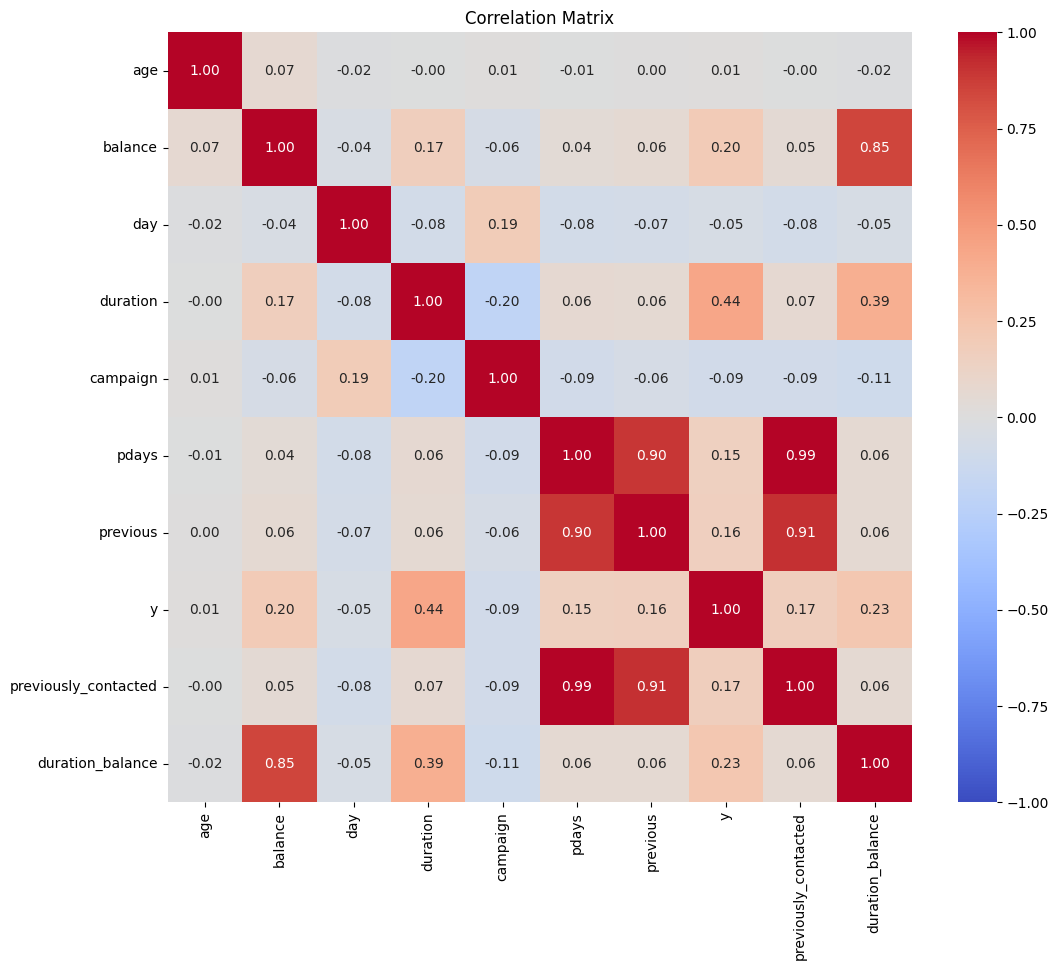
\includegraphics[width=.6\paperwidth]{./imgs/correlation_matrix.png}
\end{frame}

%------------------------------------------------
\begin{frame}{Skewed Variables}
Some variables were highly skewed:
\begin{itemize}
\item previous contacts
\item balance
\item campaign
\item duration
\end{itemize}

\centering
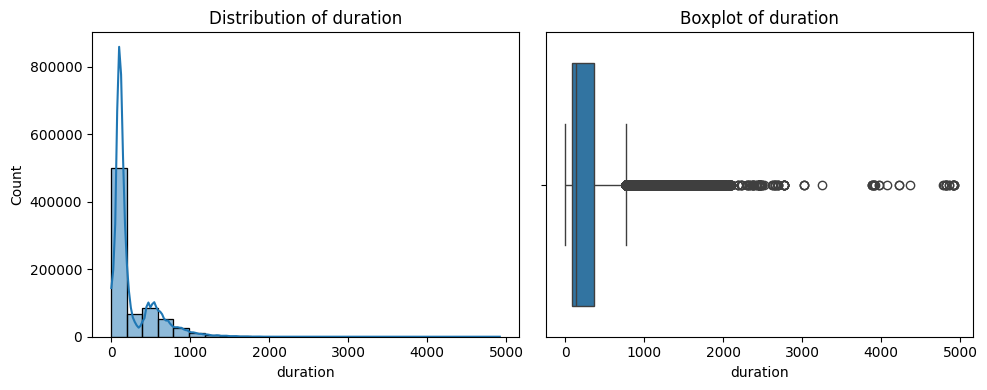
\includegraphics[width=.8\paperwidth]{./imgs/duration_skew.png}
\end{frame}

%------------------------------------------------
\begin{frame}{Feature Engineering}
Ideas implemented:
\begin{itemize}
\item Transformation for skewed data (either cube root or log1p)
\item Binary feature for previous contact (pdays == -1)
\item Interaction feature:
   \begin{itemize}
       \item job x education
       \item duration x balance
   \end{itemize}
\item Encoding categorical variables
\end{itemize}
\end{frame}

%------------------------------------------------
\begin{frame}{Encoding Strategy}

Several approaches were tested (with similar success):
\begin{itemize}
\item Label Encoding
\item Frequency Encoding
\item Target Encoding
\item Models' native category handling
\end{itemize}

\end{frame}

%------------------------------------------------
\begin{frame}{Models Tested}
\begin{itemize}
\item Random Forest baseline
\item \textbf{XGBoost} (level-wise horizontal growth: more balanced, less overfitting)
\item \textbf{LightGBM} (leaf-wise vertical growth: faster loss reduction but potential overfitting)
\item \textbf{CatBoost} (uses symmetric trees to reduce overfitting)

\end{itemize}
All evaluated with Stratified 10-fold CV.
\newline\newline{CatBoost got a major boost when it received string (categorical) features to handle natively} 
\newline\newline{For all models, a small random hyperparameter search was carried out}
\end{frame}


%------------------------------------------------
\begin{frame}{Feature Importance}
\centering
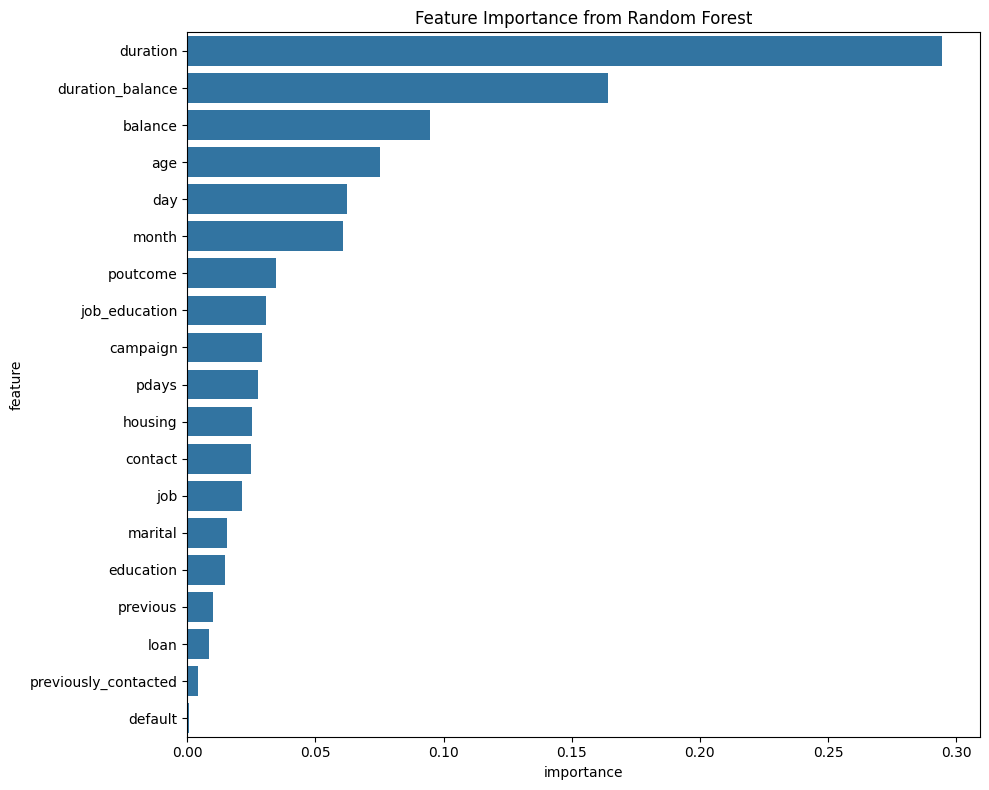
\includegraphics[width=.66\paperwidth]{./imgs/feature_importance.png}
\end{frame}

%------------------------------------------------
\begin{frame}{Model Ensemble}
Stacking method:
\begin{itemize}
\item Combine OOF predictions from:
\begin{itemize}
\item XGBoost
\item CatBoost
\item LightGBM
\end{itemize}
\item \textbf{Meta-learner}: Logistic Regression
\end{itemize}
Improves robustness and performance. It acts as a "blender", weighting the predictions of the base models to optimize final accuracy, often outperforming complex models on their own.
\end{frame}

%------------------------------------------------
\begin{frame}{Evaluation Metric}
Metric used:
\begin{itemize}
\item ROC-AUC score
\end{itemize}

Cross-validation ensures:
\begin{itemize}
\item No overfitting
\item Reliable leaderboard performance
\end{itemize}
\end{frame}

%------------------------------------------------
\begin{frame}{Results}
Final Score:
\begin{itemize}
\item ROC-AUC = 0.97478
\item Top 14\% of leaderboard
\end{itemize}

Main improvements came from:
\begin{itemize}
\item Feature engineering
\item Ensemble learning
\end{itemize}
\end{frame}

%------------------------------------------------
\begin{frame}{Lessons Learned}
\begin{itemize}
\item Feature engineering is crucial to increase AUC
\begin{itemize}
    \item Combining certain features even when the new variables are highly correlated
    \item Choosing the right encoding strategy 
    \item Tuning the model parameters
\end{itemize}
\item Tree models perform well on tabular data
\item Ensembling improves results
\end{itemize}
\end{frame}

%------------------------------------------------
\begin{frame}{References}
\begin{itemize}
\item Kaggle Bank Marketing Competition
\item Scikit-Learn documentation
\item XGBoost / LightGBM / CatBoost papers
\end{itemize}
\end{frame}

%------------------------------------------------
\begin{frame}
\centering
\Huge Thank You!
\end{frame}

\end{document}